
\documentclass[12pt]{article}
\usepackage{pifont}

\usepackage{amsmath}
\usepackage{amsfonts}
\usepackage{latexsym}
\usepackage{amssymb}
\usepackage{stmaryrd}
\usepackage{overpic}
\usepackage{graphicx}


\newtheorem{theorem}{Theorem}[section]
\newtheorem{assumption}[theorem]{Assumption}
\newtheorem{corollary}[theorem]{Corollary}
\newtheorem{definition}[theorem]{Definition}
\newtheorem{example}[theorem]{Example}
\newtheorem{lemma}[theorem]{Lemma}
\newtheorem{problem}[theorem]{Problem}
\newtheorem{proposition}[theorem]{Proposition}
\newtheorem{remark}[theorem]{Remark}
\newenvironment{proof}[1][Proof]{\textbf{#1.} }
{\ \rule{0.75em}{0.75em}\smallskip}

\renewcommand{\theequation}{\thesection.\arabic{equation}}
\renewcommand{\baselinestretch}{1.1}
\textwidth 6.5in \hoffset=-.55in \textheight=8.5in \voffset=-.65in
\parskip   1ex
\parsep    .5ex

%\usepackage{txfonts}

\begin{document}

\begin{center}
\Large\bf  A two level algorithm for an obstacle problem
\end{center}

\begin{center}
Fei Wang\footnote{Department of Mathematics, Pennsylvania State University, University Park, PA 16802, USA.}, \quad 
Joseph Eichholz\footnote{Department of Mathematics, Rose-Hulman Institute of Technology, Terre Haute, IN 47803, USA.}, 
\quad
and \quad Weimin Han\footnote{Department of Mathematics \& Program
in Applied Mathematical and Computational Sciences, University of
Iowa, Iowa City, Iowa 52242, USA.}
\end{center}

\bigskip
\begin{quote}
{\bf Abstract.}  Due to the inequality feature of the obstacle problem, the standard 
quadratic finite element method for solving the problem can only achieve an error bound
of the form ${\cal O}(N^{-3/4+\epsilon})$, $N$ being the total number of degrees of freedom,
and $\epsilon>0$ arbitrary. To achieve a better error bound, the key lies in how 
to capture the free boundary accurately. In this paper,
we propose a two level algorithm for solving the obstacle problem.
The first part of the algorithm is through the use of the linear elements on
a quasi-uniform mesh.  Then information on the approximate free boundary 
from the linear element solution is used in the construction of a quadratic finite
element method.  Under some reasonable assumptions, the numerical solution from the two
level algorithm is shown to have a nearly optimal error bound of ${\cal O}(N^{-1+\epsilon})$,
$\epsilon>0$ arbitrary. 

{\bf Keywords.} Variational inequality, free-boundary problem, quadratic elements, error estimation, optimal convergence rate

{\bf AMS Classification.} 65N30, 49J40
\end{quote}


\section{Introduction}

Many problems in physical and engineering sciences are modeled
by partial differential equations. However, various more complex 
physical processes are described by variational inequalities (VIs). 
Variational inequalities form an important family of nonlinear problems 
arising in diverse application areas, for example, elastoplasticity,
contact mechanics, heat control problems, 
options pricing problems in finance, Nash-equilibria in management science.
Therefore, how to solve variational inequalities efficiently is very attractive to 
mathematicians, engineers and economists. Variational inequalities of the first kind are 
closely related to free-boundary problems. The classical formulation of a 
variational inequality is usually expressed through the presence of an unknown 
region or boundary. So a variational inequality can be also viewed as a free-boundary
problem. Moreover, many free-boundary problems can be reformulated
as variational inequalities. The formulation of a variational inequality is advantageous 
over that of a free-boundary problem, especially for numerical solutions, since
in a variational inequality there is no explicit involvement of an unknown
region or boundary.

In this paper, we consider an obstacle problem, which is a representative 
elliptic variational inequality (EVI) of first kind (\cite{glowinski84}). 
For more examples of EVIs, we refer the reader to the monograph \cite{duvaut76}. 
Let $\Omega\subset\mathbb{R}^2$ be a bounded domain with a Lipschitz boundary $\partial\Omega$.

\noindent{\bf An obstacle problem}. Let $f\in L^2(\Omega)$, and $\psi \in H^2(\Omega)$ with $\psi \leq 0$ on $\partial\Omega$.
The obstacle problem is to find $u \in K$ such that
\begin{equation}\label{vi}
a(u,v-u) \geq (f,v-u)_\Omega \quad\forall\, v \in K,
\end{equation}
where
\begin{equation}\label{admi}
K=\{v\in H^1_0(\Omega): v\geq\psi\ {\rm a.e\ in}\ \Omega\}
\end{equation}
is a closed and convex admissible set of the space $H^1_0(\Omega)$, and
\begin{align*}
a(u,v) & =\int_\Omega \nabla u\cdot\nabla v\, dx, \\
(f,v)_\Omega &=\int_\Omega  f v \, dx. q
\end{align*}
The obstacle problem has a unique solution (\cite{duvaut76}).
It arises in a variety of
applications, such as the membrane deformation in elasticity
theory, and the non-parametric minimal and capillary surfaces as
geometrical problems. The elastic-plastic torsion problem and the
cavitation problem in the theory of lubrication also can be
regarded as obstacle type problems. If the solution has the regularity $u
\in H^2(\Omega)$, then it satisfies the relations (see, e.g., \cite{atkinson05})
\begin{equation}\label{pde}
 -\triangle u\geq f ,  \quad u\geq \psi , \quad
(-\triangle u- f)(u- \psi)=0 \quad {\rm a.e.\ in\ }\Omega.
\end{equation}
Therefore, we have the following relations
\begin{align*}
 -\triangle u &\geq f\quad {\rm in}\ \Omega^0 = \{x\in \Omega:u(x) = \psi(x)\},\\
 -\triangle u&=f\quad {\rm in}\ \Omega^+=\{x\in\Omega:u(x)>\psi(x)\}.
\end{align*}

Regarding the solution regularity of the obstacle problem, Brezis proved the
following result (see \cite{kinderlehrer80,rodrigues87}): if $\partial\Omega$ is smooth, 
$f\in L^\infty(\Omega)\cap BV(\Omega)$, and $\psi\in C^3(\bar{\Omega})$, then the 
solution of the problem \eqref{vi} has the regularity $u\in W^{s,p}(\Omega)$ with 
$1<p<\infty$ and $s<2+1/p$. 

The finite element method is the dominant numerical discretization method for 
variational inequalities. Optimal convergence order can be reached by the
linear elements (\cite{falk74, glowinski84, wang10, wang11, wang14}) under the regularity assumption 
$u\in H^2(\Omega)$.  For the quadratic element solutions, an error bound 
${\cal O}(h^{3/2-\epsilon})$, $\epsilon>0$ arbitrary, is derived for $H^1(\Omega)$-norm 
in \cite{wang02} under regularity assumption that $u\in W^{s,p}(\Omega)$ with 
$1<p<\infty$ and $s<2+1/p$.  In terms of the total number of degrees of freedom $N$, the
error bound for the linear element solution is ${\cal O}(N^{-1/2})$, whereas that for the 
quadratic element solution is ${\cal O}(N^{-3/4+\epsilon})$ for an arbitrarily small $\epsilon>0$.
For variational inequalities, higher order elements do not
lead to higher order convergence.  Therefore, it is common to use low order elements 
in solving variational inequalities.  In this paper, we introduce a two level algorithm
using both linear and quadratic elements to solve the obstacle problem such that the 
error bound is expected to be ${\cal O}(N^{-1+\epsilon})$ for an arbitrarily small $\epsilon>0$. 
In the error analysis for the two level algorithm, we adopt the assumption that 
$u\in W^{s,p}(\Omega)$ with $1<p<\infty$ and $s<2+1/p$. Moreover, we assume that 
$u|_{\Omega^0}\in H^3(\Omega^0)$ and $u|_{\Omega^+}\in H^3(\Omega^+)$, where $\Omega^0$ 
is the contact area and $\Omega^+ = \Omega\backslash \Omega^0$. 
This is a reasonable assumption. In the contact area, $u=\psi$, 
so $u|_{\Omega^0}\in H^3(\Omega^0)$ is just the assumption $\psi|_{\Omega^0}\in H^3(\Omega^0)$, 
which is implied by $\psi\in H^3(\Omega)$. $u|_{\Omega^+}\in H^3(\Omega^+)$ can be 
considered as the solution of an Poisson equation with the free-boundary as Dirichlet 
boundary condition.  The error bound is proved under some assumption on the behavior 
of the numerical solution. The idea of the algorithm is outlined as follows.  First, 
solve the obstacle problem with linear elements on a quasiuniform mesh $\mathcal{T}_h$, 
and identify free-boundary 
elements. Then refine the free-boundary elements into elements with mesh size 
$h_* = O(h^{4/3})$ to obtain a new mesh. Finally, we solve the obstacle problem on 
this new mesh with the quadratic elements. 

The rest of the paper is organized as follows: In Section \ref{sec:alg}, we introduce
the two level  algorithm. In Section \ref{sec:est}, we derive a priori error
estimates for this algorithm.  In Section \ref{sec:num}, we present numerical examples to 
provide numerical evidence of the error bound.  



\section{A two level algorithm}\label{sec:alg}
\setcounter{equation}0

We assume $\Omega$ is a polygonal domain.  For a subdivision ${\cal T}_h$ of
$\overline{\Omega}$ into triangles, let $h_T ={\rm diam}(T)$ and $h =
\max\{h_T: T\in \mathcal{T}_h\}$.  All the subdivisions, including the refined meshes,
are constructed so that the minimal angle condition is satisfied.


We introduce the following two level quadratic finite element method for the obstacle problem.
\begin{enumerate}
\item[1] Solve the obstacle problem on a quasi-uniform mesh $\mathcal{T}_h$ with the linear elements, 
that is, find $u_h \in K_h^1$ such that
\begin{equation}\label{dvi_1}
a(u_h,v_h-u_h) \geq (f,v_h-u_h)_\Omega \quad\forall\,v_h \in K_h^1,
\end{equation}
where
\[ K_h^1 = \{ v_h \in V_h^1: \; v_h(x) \geq \psi(x)\ {\rm at\ all\ vertices\ of}\ \mathcal{T}_h\} \]
and 
\[ V_h^1 =\{v_h \in H^1(\Omega): \;v_h |_T \in P_1(T)\
\forall\,T\in\mathcal{T}_h   \}. \]
\item[2] Identify the subset $\mathcal{T}_h^F\subset\mathcal{T}_h$ of free-boundary elements, 
i.e., the subset of the elements $T\in{\cal T}_h$ such that $T=T_1\cup T_2$ with $|T_1|>0$, 
$|T_2|>0$, $u_h=\psi$ on $T_1$, and $u_h>\psi$ on $T_2$.  
Refine all the elements in $\mathcal{T}_h^F$ into new elements 
with mesh size $h_*=O(h^{4/3})$.  Denote the new mesh by ${\cal T}_h^*$.
\item Solve the obstacle problem with quadratic elements over the new mesh $\mathcal{T}_h^*$, 
i.e., find $u_h^* \in K_h^2$ such that
\begin{equation}\label{dvi_2}
a(u_h^*,v_h-u^*_h) \geq (f,v_h-u^*_h)_\Omega \quad\forall\,v_h \in K_h^2,
\end{equation}
where
\[ K_h^2 = \{ v_h \in V_h^2: \; v_h(m) \geq \psi(m)\ {\rm at\ all\
midpoints}\ m\ {\rm on\ element \ edges\ of}\ \mathcal{T}_h^*\} \]
and
\[ V_h^2=\{v_h \in H^1(\Omega): \;v_h |_T \in P_2(T)\ \forall\,T\in\mathcal{T}_h^*  \}. \]
In the iterative procedure for solving the problem \eqref{dvi_2}, for the initial guess 
we use the interpolant of $u_h$ in $V_h^2$.
\end{enumerate}

In the next section, under the solution smoothness assumption $v\in V$, where  
\begin{align}
V&=\{v\in W^{s,p}(\Omega):\; v|_{\Omega^0}\in H^3(\Omega^0)
 \ {\rm and}\ v|_{\Omega^+}\in H^3(\Omega^+)\}\label{regularity}
\end{align}
with $1<p<\infty$ and $s<2+1/p$, and a natural assumption on the numerical solution, we will prove 
that for the two level algorithm, $\|u-u^*_h\|_1\leq C h^{2-\epsilon}$; or, in terms
of the total number of degrees of freedom $N$, $\|u-u^*_h\|_1\leq C N^{-1+\epsilon}$.

\section{Error estimates}\label{sec:est}
\setcounter{equation}0

First recall the following boundedness and stability properties of the bilinear form $a(u,v)$.

\begin{lemma}
\begin{align}\label{bound}
a(u,v)&\leq C_b  \|u\|_1\| v\|_1\quad\forall\, u,v \in H^1_0(\Omega),\\
a(v,v)&\geq C_s \|v\|_1^2 \quad \forall\, v \in H^1_0(\Omega),
\label{stable}
\end{align}
where $C_b$ and $C_s$ are positive constants independent of the mesh size.
\end{lemma}


The main purpose of the section is to bound the error for the two level method. 
We assume $u\in V$.  Let us group the elements of $\mathcal{T}_h^*$ into three kinds:
\begin{align*}
  \mathcal{T}_h^+ &= \{T\in \mathcal{T}_h^*: T \subset \Omega^+\}, \\
  \mathcal{T}_h^0 &= \{T\in \mathcal{T}_h^*: T \subset \Omega^0\}, \\
  \mathcal{T}_h^b &= \mathcal{T}_h^* \backslash(\mathcal{T}_h^+\cup\mathcal{T}_h^0).
\end{align*}
We will assume 
\begin{equation}
 \bigcup_{T\in \mathcal{T}_h^b} T\subset \bigcup_{T\in\mathcal{T}_h^F} T,
\label{assumpT}
\end{equation}
where $\mathcal{T}_h^F$ was defined in Step 2 of the algorithm.
This is a reasonable assumption if $h$ is small enough, given the first order convergence
of $u_h$ to $u$ in $H^1(\Omega)$.  Write the error as
\[e = u - u_h^* = (u - u_I) + (u_I - u_h^*),\]
where $u_I \in V_h^2$ is the usual continuous piecewise quadratic polynomial
interpolant.   Then
\begin{equation}\label{gappro}
\|u-u_I\|_1  \lesssim h^{2-\epsilon},
\end{equation}
where ``$\lesssim\cdots $" stands for ``$\leq C\cdots $", and $C$
is a positive generic constant independent of $h$ and other
parameters, which may take different values at different appearances.
In fact, because $u|_{\Omega^0}\in H^3(\Omega^0)$ and $u|_{\Omega^+}\in H^3(\Omega^+)$, 
for any $T\in \mathcal{T}_h^0\cup\mathcal{T}_h^+$, we have 
\[\|u-u_I\|_{1,T} \leq C h^2 |u|_{3,T},\] 
and for any $T\in \mathcal{T}_h^b$, we have 
\[\|u-u_I\|_{1,T} \leq C h_*^{3/2-3\epsilon/4} |u|_{5/2-3\epsilon/4,T}
 \leq C h^{2-\epsilon} |u|_{5/2-3\epsilon/4,T},\]
with $s=5/2-3\epsilon/4<2+1/p$, $p=2$ in \eqref{regularity}.

Using a technique similar to that in \cite{wang02, wang10}, we derive the following error estimate.

\begin{theorem}\label{thm1qua}
Let $u$ and $u_h^*$ be the solutions of \eqref{vi} and \eqref{dvi_2}, respectively. 
Assume $u\in V$ defined in \eqref{regularity}, $\psi\in H^3(\Omega)$, $f\in H^1(\Omega)\cap L^\infty(\Omega)$, 
and \eqref{assumpT}.  Then for the two level method introduced in Section \ref{sec:alg}, we have
\begin{equation} \label{errh}
\|u-u_h^*\|_1 \leq C h^{2-\epsilon},
\end{equation}
for an arbitrary $\epsilon>0$.
\end{theorem}
\begin{proof}
By the stability of the bilinear form $a(u,v)$, we have
\begin{equation}
C_s\|u_I-u_h^*\|_1^2 \le a(u_I-u_h^*,u_I-u_h^*)\equiv A_1+A_2, \label{err1qua}
\end{equation}
where
\begin{align*}
A_1 &= a(u_I-u,u_I-u_h^*),\\
A_2&= a(u-u_h^*,u_I-u_h^*).
\end{align*}
By the boundedness of the bilinear form, the term $A_1$ is bounded by
\begin{equation}
  A_1 \leq C_b\|u_I-u\|_1\|u_I-u_h^*\|_1
   \le \frac{C_s}{2}\|u_I-u_h^*\|_1^2
    +\frac{C_b^2}{2C_s}\|u_I-u\|_1^2.
\label{err2qua}
\end{equation}

To bound $A_2$, we first recall the relations
\begin{align*}
 -\triangle u&=f\quad {\rm in}\ \Omega^+=\{x\in\Omega:u(x)>\psi(x)\},\\
 -\triangle u &\geq f\quad {\rm in}\ \Omega^0 = \{x\in \Omega:u(x) = \psi(x)\}.
\end{align*}
Note that $u_I - u_h^*=0$ on $\partial\Omega$.  We have
\begin{align}\label{1}
a(u,u_I-u_h^*)&=\int_\Omega\nabla u\cdot\nabla(u_I-u_h^*)\,dx=-\int_\Omega \Delta u (u_I-u_h^*)\,dx.
\end{align}
Let $v_h = u_I$ in (\ref{dvi_2}),
\begin{equation}\label{2}
  a(u_h^*,u_I-u_h^*) \ge (f,u_I-u_h^*)_\Omega = \sum_{T\in \mathcal{T}_h}\int_T f
  (u_I-u_h^*)\, dx.
\end{equation}
Combining (\ref{2}) and (\ref{1}), we obtain
\begin{equation}\label{T2}
A_2=a(u-u_h^*,u_I-u_h^*) \le\sum_{T\in \mathcal{T}_h}\int_T -(\Delta u+ f)(u_I-u_h^*)\,dx
\equiv A_3+A_4+A_5, 
\end{equation}
where
\begin{align*}
A_3 &= \sum_{T\in \mathcal{T}_h^+}\int_T w(u_I-u_h^*)\, dx, \\
A_4 & = \sum_{T\in \mathcal{T}_h^0}\int_T w(u_I-u_h^*)\, dx, \\
A_5 & = \sum_{T\in \mathcal{T}_h^b}\int_T w(u_I-u_h^*)\, dx.
\end{align*}
Here, we denote $w:=-\Delta u - f$. It is easy to see that $A_3=0$.

To estimate $A_4$, as in \cite{wang02}, we introduce
\[P^T_0 v = \frac{1}{|T|}\int_T v\,dx,\quad\quad  R^T_0 v = v - P^T_0 v.\]
Since $w\geq 0$, we get $P^T_0 w \geq 0$. Due to $u_h^*\in K_{h}^2$, we have
$u_h^*(m)\geq \psi(m)$ for all the midpoints $m$ on the edges of the element
$T$, implying
\[ \int_T (\psi_I - u_h^*)\,dx=\frac{|T|}{3}\sum_{i=1}^3 (\psi - u_h^*)(m_i)\leq 0. \]
Then we get
\begin{align*}
\int_T w(\psi_I - u_h^*)\,dx & \leq \int_T R^T_0 w(\psi_I - u_h^*)\,dx\\
&=\int_T R^T_0 w \, R^T_0(\psi_I - u_h^*)\,dx \leq \|R^T_0
w\|_{0,T}\|R^T_0(\psi_I - u_h^*)\|_{0,T}.
\end{align*}
Note that $u=\psi$ in $T \in \mathcal{T}_h^0$ and $\psi\in H^3(\Omega)$; so
\begin{align*}
\int_T w(\psi_I - u_h^*)\,dx &\leq C h^2 |w|_{1,T}|\psi_I-u_h^*|_{1,T}\\
&\leq C h^2 |w|_{1,T}(|\psi_I-\psi|_{1,T}+|\psi-u|_{1,T}+|u- u_h^*|_{1,T}).
\end{align*}
We then apply interpolation error estimates to get
\begin{equation}
\int_T w(\psi_I - u_h^*)\,dx 
\leq C h^2 |w|_{1,T}(h^2|\psi|_{3,T}+|u-u_h^*|_{1,T}).
\label{3.8a}
\end{equation}
Hence,
\begin{equation}\label{err3qua}
A_4 = \sum_{T\in \mathcal{T}_h^0}\int_T w(\psi_I-u_h^*)\, dx 
\leq C h^2 |w|_{1,\Omega}(h^2|\psi|_{3,\Omega}+\|u-u_h^*\|_1).
\end{equation}

Consider the term 
\begin{align*}
A_5=\sum_{T\in \mathcal{T}_h^b} \int_T w (u_I-u+\psi-\psi_I)dx 
+ \sum_{T\in \mathcal{T}_h^b} \int_T w (u-\psi)dx
  +\sum_{T\in \mathcal{T}_h^b} \int_T w (\psi_I-u_h^*)dx.
\end{align*}
Since $w (u-\psi)=0$ by (\ref{pde}), we can write
\[ A_5=A_{5,1}+A_{5,2},\]
where
\begin{align*}
A_{5,1}&=\sum_{T\in \mathcal{T}_h^b} \int_T  w [(u-\psi)_I-(u-\psi)]dx,\\
A_{5,2}&=\sum_{T\in \mathcal{T}_h^b} \int_T w (\psi_I-u_h^*)dx.
\end{align*}
Using a technique similar to that in \cite{brezzi77}, we can bound the
term $A_{5,1}$ as follows:
\begin{align}
A_{5,1} &\lesssim  h^{4-\epsilon} \|w\|_{L^\infty(\Omega)} \|u-\psi\|_{s,p,\Omega}. \label{errorA51}
\end{align}
Indeed, for any $v\in W^{s,p}(\Omega)$ with $1<p<\infty$ and $s<2+1/p$, by the Cauchy-Schwarz 
inequality and the interpolation error estimate, we get 
\[\|v_I-v\|_{0,1,T} = \int_T |v_I-v|\, dx \leq |T|^{1-\frac{1}{p}} \|v_I-v\|_{0,p,T}
\lesssim h_*^{s+2-\frac{2}{p}}\|v\|_{s,p,T}, \]
and then,
\begin{align*}
\sum_{T\in \mathcal{T}_h^b} \|v_I-v\|_{0,1,T} 
& \lesssim h_*^{s+2-\frac{2}{p}} \sum_{T\in \mathcal{T}_h^b} \|v\|_{s,p,T} \\
& \lesssim h_*^{s+2-\frac{2}{p}} \left(\sum_{T\in \mathcal{T}_h^b} 1\right)^{1-\frac{1}{p}}
  \left(\sum_{T\in \mathcal{T}_h^b} \|v\|_{s,p,T}^p\right)^{\frac{1}{p}}\\
& \lesssim h_*^s \|v\|_{s,p,\Omega}. 
\end{align*}
Hence,
\begin{align*}
A_{5,1}&=\sum_{T\in \mathcal{T}_h^b} \int_T  w [(u-\psi)_I-(u-\psi)]dx\\ 
& \leq \|w\|_{L^\infty(\Omega)} \sum_{T\in \mathcal{T}_h^b} \|(u-\psi)_I-(u-\psi)\|_{0,1,T} \\
& \lesssim h_*^s \|w\|_{L^\infty(\Omega)} \|u-\psi\|_{s,p,\Omega}. 
\end{align*}
Taking $p = 1 + \epsilon_1$, $s = 2 + \frac{1}{p} - \epsilon_2 = 3 - 3\epsilon/4$, with 
$\epsilon = \frac{4}{3}\left(\frac{\epsilon_1}{1+\epsilon_1} + \epsilon_2\right)$ in the 
above inequality, and note that $h_*=O(h^{4/3})$, we get the bound \eqref{errorA51}
for the term $A_{5,1}$.

Finally, let us bound the term $A_{5,2}$. We know that
\begin{align}
\int_T w(\psi_I - u_h^*)\,dx &\leq \int_T R^T_0 w \, R^T_0(\psi_I - u_h^*)\,dx \nonumber\\
& =\int_T R^T_0 w \, [R^T_0(\psi_I -\psi) + R^T_0(\psi - u) + R^T_0(u - u_h^*)]\,dx.\label{A52}
\end{align}
By interpolation error estimate, for the first and third terms on the right hand side of \eqref{A52}, we have
\begin{align*}
\sum_{T\in \mathcal{T}_h^b} \int_T R^T_0 w \, R^T_0(\psi_I -\psi) \,dx  
&\leq \sum_{T\in \mathcal{T}_h^b} \|R^T_0 w\|_{0,T} \|R^T_0(\psi_I -\psi)\|_{0,T}\\
&\leq  C \sum_{T\in \mathcal{T}_h^b} h_*^{3/2-3\epsilon/4}  \|w\|_{1/2-3\epsilon/4, T}|\psi_I -\psi|_{1,T} \\
&\leq C \sum_{T\in \mathcal{T}_h^b} h_*^{7/2-3\epsilon/4}   \|w\|_{1/2-3\epsilon/4, T}|\psi|_{3,T}\\ 
&\leq  C \sum_{T\in \mathcal{T}_h^b} h^{\frac{14}{3}-\epsilon}   \|w\|_{1/2-3\epsilon/4, T}|\psi|_{3,T}\\
&\leq C h^{\frac{14}{3}-\epsilon}   \|w\|_{1/2-3\epsilon/4, \Omega}|\psi|_{3,\Omega}, 
\end{align*}
and
\begin{align*}
\sum_{T\in \mathcal{T}_h^b} \int_T R^T_0 w \, R^T_0(u - u_h^*) \,dx  
&\leq \sum_{T\in \mathcal{T}_h^b} \|R^T_0 w\|_{0,T} \|R^T_0(u - u_h^*)\|_{0,T}\\
&\leq  C \sum_{T\in \mathcal{T}_h^b} h_*^{3/2-3\epsilon/4}  \|w\|_{1/2-3\epsilon/4, T}|u - u_h^*|_{1,T} \\
&\leq C \sum_{T\in \mathcal{T}_h^b} h^{2-\epsilon}   \|w\|_{1/2-3\epsilon/4, T}|u - u_h^*|_{1,T}\\ 
&\leq  C  h^{2-\epsilon}   \|w\|_{1/2-3\epsilon/4, \Omega}|u - u_h^*|_{1,\Omega}.
\end{align*}
Next we bound the second term on the right hand side of \eqref{A52}.
\begin{align*}
\int_T R^T_0 w \, R^T_0(\psi - u) \,dx 
& \leq \|R^T_0 w\|_{0,1,T} \|R^T_0(\psi - u)\|_{0,\infty,T}\\
&\leq  |T|^{1-\frac{1}{p}} \|R^T_0 w\|_{0,p,T} \|R^T_0(\psi - u)\|_{0,\infty,T}\\
&\leq C h_*^{3-\frac{1}{p}-\epsilon_1}\|w\|_{\frac{1}{p}-\epsilon_1,p,T}|\psi-u|_{1,\infty,T}.
\end{align*}
Now, we need to estimate $|\psi-u|_{1,\infty,T}$ for
any $T\in \mathcal{T}_h^b$.  From the assumption
$\psi \in H^3(\Omega)$ and $u\in V$, we know that 
\[\nabla(\psi-u) \in W^{1+1/t-\epsilon_2,t}(\Omega)
\hookrightarrow C^{0,\alpha}(\Omega),\ {\rm with}\ \alpha = 1-1/t-\epsilon_2.\] 
By the assumption \eqref{assumpT}, since $T \in \mathcal{T}_h^b$, there is 
a point $Q\in T$ such that $\nabla(\psi -u)(Q) = 0$. Then for any $x\in T\in \mathcal{T}_h^b$, 
we have
\begin{align*}
|\nabla(\psi-u)(x)|& =|\nabla(\psi-u)(x)-\nabla(\psi - u)(Q)|\\
  &\leq  C |x-Q|^\alpha\|\psi-u\|_{2+1/t-\epsilon_2,t,\Omega} \\
  &\leq C h_*^\alpha\|\psi-u\|_{2+1/t-\epsilon_2,t,\Omega}. 
\end{align*}
Thus,
\[ |\psi -u|_{1,\infty,T}\leq C h_*^\alpha \|\psi-u\|_{2+1/t-\epsilon_2,t,\Omega}.\]
Then
\begin{align*}
\sum_{T\in \mathcal{T}_h^b}  \int_T R^T_0 w \, R^T_0(\psi - u) \,dx 
&\leq C h_*^{\alpha+3-\frac{1}{p}-\epsilon_1}
\left(\sum_{T\in \mathcal{T}_h^b}\|w\|_{\frac{1}{p}-\epsilon_1,p,T}\right) \|\psi-u\|_{2+1/t-\epsilon_2,t,\Omega}\\
&\leq  C h_*^{\alpha+3-\frac{1}{p}-\epsilon_1} \left(\sum_{T\in \mathcal{T}_h^b} 1\right)^{1-\frac{1}{p}} 
 \|w\|_{\frac{1}{p}-\epsilon_1,p,\Omega} \|\psi-u\|_{2+1/t-\epsilon_2,t,\Omega} \\
&\leq C h_*^{3-\epsilon} \|w\|_{\frac{1}{p}-\epsilon_1,p,\Omega} \|\psi-u\|_{2+1/t-\epsilon_2,t,\Omega} ,
\end{align*}
where $\alpha = 1-1/t-\epsilon_2$, $\epsilon_3 = 1/t$, $p=1+\epsilon_1$, and 
$\epsilon=\frac{\epsilon_1(2+\epsilon_1)}{1+\epsilon_1} + \epsilon_2+ \epsilon_3>0$.
Note that $h_*=O(h^{4/3})$, we obtain
\begin{align*}
\sum_{T\in \mathcal{T}_h^b}  \int_T R^T_0 w \, R^T_0(\psi - u) \,dx 
&\leq h^{4-\epsilon} \|w\|_{\frac{1}{p}-\epsilon_1,p,\Omega} \|\psi-u\|_{2+1/t-\epsilon_2,t,\Omega} .
\end{align*}
The proof is completed then.
\end{proof}

Suppose the free boundary is a ``regular" curve.  Then there are ${\cal O}(h^{-1})$
elements to be refined to smaller size, and the number of smaller size elements
will be ${\cal O}(h^{-5/3})$.  Thus, after the refinement, there are ${\cal O}(h^{-2})$ 
elements of the size $h$, and ${\cal O}(h^{-5/3})$ elements of the size $h^*$.
So the total number of elements is ${\cal O}(h^{-2})$, which means that the total degrees of
freedom do not increase significantly compared to the standard quadratic element on mesh 
$\mathcal{T}_h$. Let $N$ be the number of degrees of freedom for the linear element 
space $V_h^1$.  Then the error bound \eqref{errh} implies that
\[ \|u-u_h^*\|_1 \leq C \, N^{-1+\epsilon}, \]
instead of obtaining convergence rate ${\cal O}(N^{-3/4+\epsilon})$ in \cite{wang02}. This two level
algorithm can also applied to other variational inequalities of the first kind.

\section{Numerical examples}\label{sec:num}
\setcounter{equation}0

In this section, we give two numerical examples to test the two level algorithm described in Section \ref{sec:alg}.

To implement the second step in the algorithm, we first need
to find the free boundary elements of $\mathcal{T}_h$.  An element $T\in
  \mathcal{T}_h$ is said to be a free boundary element if there exist vertices
  $v_1$ and $v_2$ of $T$ such that $u_h(v_1)=\psi(v_1)$ and
  $u_h(v_2)>\psi(v_2)$. Let the set of free boundary elements of
  $\mathcal{T}_h$ be denoted by $\mathcal{T}_h^F$. 
Then, create a new mesh of $\Omega$, $\mathcal{T}_h^*$, by refining all the
  elements in $\mathcal{T}_h^F$.  Denote the refinement of $\mathcal{T}_h^F$ as $\mathcal{T}_*^F$.
Let $h^F$ and $h_*^F$ be the maximal edge lengths in $\mathcal{T}_h^F$ and $\mathcal{T}_*^F$, respectively.   
We choose a \textit{mesh refinement parameter} $C$, and  ensure that we refine $T_h^F$ enough times to respect
the \textit{mesh refinement criterion}
  \begin{equation}
    \label{eq:mesh-refinement-criteria}
    h_*^F\le C \left(h^F\right)^{4/3}.
  \end{equation}
In particular, if we use the simple red-green refinement approach for
a two-dimensional mesh, we refine every element of $\mathcal{T}_h^F$ by $\max\left(1,\left\lceil
-\log_2\left(C \left(h^F\right)^{1/3}\right)\right\rceil\right)$ times. 
The elements $T \notin T_h^F$ are left unrefined, except in the case that they must be refined 
in order to avoid hanging nodes.   

We test the two level algorithm on two examples,
comparing the method with the standard linear and quadratic finite
element method, as well as an algorithm in which we simply
refine the free boundary mesh $\mathcal{T}_h^F$ one time rather than respecting
the mesh refinement criterion \eqref{eq:mesh-refinement-criteria}.  We
shall refer to the two level algorithm which does not respect
\eqref{eq:mesh-refinement-criteria} as the \textit{non-respecting}
refinement method, and the two level algorithm which does respect
\eqref{eq:mesh-refinement-criteria} as the refinement method. 

\subsection{Example 1}
Consider the obstacle problem \eqref{vi}--\eqref{admi} in the domain $\Omega=(-1.5,1.5)^2$ with 
a constant right hand side term $f(x)= -2$ and the obstacle function $\psi(x)=0$. Given the boundary
condition $u_0(r)=\frac{r^2}{2}-\ln(r)-1/2$, the exact solution to \eqref{vi}--\eqref{admi} is
\begin{equation*}
u(r)=  \begin{cases}
  0 &\text{ if } r<1,\\
  \frac{r^2}{2}-\ln(r)-1/2 & \text{ otherwise.}
\end{cases}
\end{equation*}

In the numerical examples we choose the mesh refinement parameter $C=10$.  
In Figures \ref{fig:example1-error}--\ref{fig:example1-time} we compare the
accuracy of each of the four numerical methods, as well as the time
required to compute each solution.  We can see that the two level
method outperforms the two standard methods in both regards.  As expected,
the non-respecting two level method does not converge as rapidly as the two level method. 




% \begin{figure}
% \centering
% \includegraphics[width=4in]{example1/Error.pdf}
% \caption{Degrees of freedom vs.\ $H^1$ error for Example 1.}
% \label{fig:example1-error}
% \end{figure}

% \begin{figure}
% \centering
% \includegraphics[width=4in]{example1/ErrorH.pdf}
% \caption{Mesh size vs.\ $H^1$ error for Example 1.}
% \label{fig:example1-herror}
% \end{figure}


% \begin{figure}
% \centering
% \includegraphics[width=4in]{example1/ComputingTime.pdf}
% \caption{Solution time (s) vs.\ $H^1$ error for Example 1.}
% \label{fig:example1-time}
% \end{figure}



\begin{table}
\begin{tabular}{|r|r|r|r|r|r|}
\hline
$N$&$h$&$H^1$ Error&$N$ Conv.\ Rate &$h$ Conv.\ Rate&Comp.\ Time (s)\\ 
\hline
\hline
17&1.677e+00&1.207e+00&-&-&1.702e-02\\ 
31&1.008e+00&7.486e-01&7.945e-01&9.372e-01&2.441e-02\\ 
101&5.252e-01&3.527e-01&6.371e-01&1.155e+00&2.242e-02\\ 
366&2.650e-01&1.800e-01&5.225e-01&9.835e-01&3.748e-02\\ 
1385&1.325e-01&9.085e-02&5.138e-01&9.868e-01&8.349e-02\\ 
5308&6.629e-02&4.588e-02&5.085e-01&9.862e-01&3.210e-01\\ 
20958&3.315e-02&2.292e-02&5.055e-01&1.002e+00&1.850e+00\\ 
83087&1.657e-02&1.146e-02&5.029e-01&9.993e-01&1.612e+01\\ 
330653&8.286e-03&5.749e-03&4.997e-01&9.956e-01&1.912e+02\\ 
\hline
\end{tabular}
\caption{Results for linear method in Example 1.}
\label{tab:example1-linear}
\end{table}

\begin{table}
\begin{tabular}{|r|r|r|r|r|r|}
\hline
$N$&$h$&$H^1$ Error&$N$ Conv.\ Rate &$h$ Conv.\ Rate&Comp.\ Time (s)\\ 
\hline
\hline
49&1.677e+00&5.900e-01&-&-&2.254e-02\\ 
105&1.008e+00&1.390e-01&1.897e+00&2.839e+00&2.635e-02\\ 
369&5.252e-01&7.419e-02&4.995e-01&9.632e-01&3.873e-02\\ 
1397&2.650e-01&2.064e-02&9.611e-01&1.871e+00&6.350e-02\\ 
5409&1.325e-01&7.199e-03&7.780e-01&1.520e+00&2.188e-01\\ 
20973&6.629e-02&2.639e-03&7.406e-01&1.449e+00&1.941e+00\\ 
83317&3.315e-02&9.073e-04&7.739e-01&1.540e+00&1.984e+01\\ 
331319&1.657e-02&3.206e-04&7.536e-01&1.501e+00&2.498e+02\\ 
1320561&8.286e-03&1.122e-04&7.590e-01&1.514e+00&2.791e+03\\ 
\hline
\end{tabular}
\caption{Results for quadratic method in Example 1.}
\label{tab:example1-quadratic}
\end{table}

\begin{table}
\begin{tabular}{|r|r|r|r|r|r|}
\hline
$N$&$h$&$H^1$ Error&$N$ Conv.\ Rate &$h$ Conv.\ Rate&Comp.\ Time (s)\\ 
\hline
\hline
137&1.677e+00&2.050e-01&-&-&1.153e-01\\ 
320&1.008e+00&6.373e-02&1.377e+00&2.295e+00&7.576e-02\\ 
815&5.252e-01&2.825e-02&8.701e-01&1.248e+00&1.096e-01\\ 
2413&2.650e-01&8.183e-03&1.142e+00&1.812e+00&1.325e-01\\ 
7185&1.325e-01&3.106e-03&8.877e-01&1.398e+00&3.440e-01\\ 
24593&6.629e-02&1.190e-03&7.798e-01&1.385e+00&1.151e+00\\ 
90277&3.315e-02&4.474e-04&7.523e-01&1.411e+00&5.704e+00\\ 
345815&1.657e-02&1.512e-04&8.077e-01&1.565e+00&3.733e+01\\ 
1349265&8.286e-03&5.192e-05&7.851e-01&1.542e+00&3.279e+02\\ 
\hline
\end{tabular}
\caption{Results for refinement (non-respecting) method in Example 1.}
\label{tab:example1-adaptiveno43}
\end{table}

\begin{table}
\begin{tabular}{|r|r|r|r|r|r|}
\hline
$N$&$h$&$H^1$ Error&$N$ Conv.\ Rate &$h$ Conv.\ Rate&Comp.\ Time (s)\\ 
\hline
\hline
137&1.677e+00&2.050e-01&-&-&7.699e-02\\ 
320&1.008e+00&6.373e-02&1.377e+00&2.295e+00&8.188e-02\\ 
815&5.252e-01&2.825e-02&8.701e-01&1.248e+00&9.927e-02\\ 
2413&2.650e-01&8.183e-03&1.142e+00&1.812e+00&1.558e-01\\ 
13725&1.325e-01&1.481e-03&9.834e-01&2.467e+00&6.389e-01\\ 
80125&6.629e-02&3.434e-04&8.283e-01&2.110e+00&5.474e+00\\ 
196377&3.315e-02&1.099e-04&1.271e+00&1.644e+00&1.871e+01\\ 
1147579&1.657e-02&2.388e-05&8.646e-01&2.202e+00&2.205e+02\\ 
\hline
\end{tabular}
\caption{Results for refinement (respecting) method in Example 1.}
\label{tab:example1-adaptive}
\end{table}


We report the same results in tabular form in Tables \ref{tab:example1-linear}--\ref{tab:example1-adaptive}.  
In addition, for each method we compute the numerical convergence orders.  In particular, let $N_i$ 
denote the number of degrees of freedom corresponding to the $i^{th}$ approximation. Let $h_i$ denote the
largest edge length from the mesh $\mathcal{T}^i_h$, and define $E_i$ as the
$H^1(\Omega)$ error achieved by approximation $i$. The convergence rate in the term of $N$ refers to 
$\alpha$ in $O(N^{-\alpha})$, and we estimate the order of convergence in terms of $N$ for the methods 
by $\alpha\approx -\frac{\log(E_i/E_{i-1})}{\log(N_i/N_{i-1})}$. We estimate the order of
convergence in terms of $h$ via $p\approx\frac{\log(E_i/E_{i-1})}{\log(h_i/h_{i-1})}$.  

In Tables \ref{tab:example1-linear}--\ref{tab:example1-adaptive} we can see
each method tending toward its expected order of convergence. 


\subsection{Example 2}
As in Example 1, let the domain be $\Omega=[-2,2]^2$. Define $f(x)=0$ and obstacle function as
\begin{align*}
  &\psi(r)=\begin{cases}\sqrt{1-r^2}&\text{ if } r<1, \\
                                  0&\text{otherwise}\end{cases}.\label{ex2-f}
\end{align*}
The boundary condition is given as 
\[ u_0(r)=-\left(r^*\right)^2\frac{\ln(r/2)}{\sqrt{1-\left(r^*\right)^2}} \label{ex2-u0}, \]
where $r=\sqrt{x_1^2+x_2^2}$ and $r^*=0.6979651482$.
Then, the exact solution to \eqref{vi}--\eqref{admi} is
\begin{equation*}
u(r)=  \begin{cases}
  \sqrt{1-r^2} &\text{ if } r<r^*,\\
  -\left(r^*\right)^2\frac{\ln(r/2)}{\sqrt{1-\left(r^*\right)^2}} & \text{ otherwise} .
\end{cases}
\end{equation*}


% \begin{figure}
% \centering
% \includegraphics[width=4in]{example2/Error.pdf}
% \caption{Degrees of freedom vs.\ $H^1$ error for Example 2.}
% \label{fig:example2-error}
% \end{figure}

% \begin{figure}
% \centering
% \includegraphics[width=4in]{example2/ErrorH.pdf}
% \caption{Mesh size vs.\ $H^1$ error for Example 2.}
% \label{fig:example2-herror}
% \end{figure}


% \begin{figure}
% \centering
% \includegraphics[width=4in]{example2/ComputingTime.pdf}
% \caption{Solution time (s) vs.\ $H^1$ error for Example 2.}
% \label{fig:example2-time}
% \end{figure}


\begin{table}
\begin{tabular}{|r|r|r|r|r|r|}
\hline
$N$&$h$&$H^1$ Error&$N$ Conv.\ Rate &$h$ Conv.\ Rate&Comp. Time (s)\\ 
\hline
\hline
17&1.677e+00&5.765e-01&-&-&2.194e-02\\ 
31&1.008e+00&7.005e-01&-3.244e-01&-3.827e-01&3.161e-02\\ 
101&5.252e-01&3.386e-01&6.154e-01&1.115e+00&3.797e-02\\ 
366&2.650e-01&1.666e-01&5.508e-01&1.037e+00&6.497e-02\\ 
1385&1.325e-01&8.278e-02&5.257e-01&1.010e+00&1.203e-01\\ 
5308&6.629e-02&4.216e-02&5.022e-01&9.740e-01&3.451e-01\\ 
20958&3.315e-02&2.124e-02&4.991e-01&9.889e-01&1.814e+00\\ 
83087&1.657e-02&1.065e-02&5.016e-01&9.968e-01&1.641e+01\\ 
330653&8.286e-03&5.327e-03&5.013e-01&9.990e-01&1.992e+02\\ 
\hline
\end{tabular}
\caption{Results for linear method in Example 2.}
\label{tab:example2-linear}
\end{table}


\begin{table}
\begin{tabular}{|r|r|r|r|r|r|}
\hline
$N$&$h$&$H^1$ Error&$N$ Conv.\ Rate &$h$ Conv.\ Rate&Comp.\ Time (s)\\ 
\hline
\hline
49&1.677e+00&6.289e-01&-&-&2.993e-02\\ 
105&1.008e+00&1.520e-01&1.864e+00&2.789e+00&3.435e-02\\ 
369&5.252e-01&7.797e-02&5.310e-01&1.024e+00&5.610e-02\\ 
1397&2.650e-01&3.447e-02&6.132e-01&1.194e+00&1.011e-01\\ 
5409&1.325e-01&1.225e-02&7.640e-01&1.493e+00&3.084e-01\\ 
20973&6.629e-02&4.679e-03&7.103e-01&1.389e+00&1.648e+00\\ 
83317&3.315e-02&1.549e-03&8.015e-01&1.595e+00&1.824e+01\\ 
331319&1.657e-02&5.615e-04&7.351e-01&1.464e+00&2.462e+02\\ 
1320561&8.286e-03&1.973e-04&7.565e-01&1.509e+00&3.153e+03\\ 
\hline
\end{tabular}
\caption{Results for quadratic method in Exampl 2.}
\label{tab:example2-quadratic}
\end{table}


\begin{table}
\begin{tabular}{|r|r|r|r|r|r|}
\hline
$N$&$h$&$H^1$ Error&$N$ Conv.\ Rate &$h$ Conv.\ Rate&Comp.\ Time (s)\\ 
\hline
\hline
137&1.677e+00&1.459e-01&-&-&7.092e-02\\ 
314&1.008e+00&9.188e-02&5.573e-01&9.076e-01&8.227e-02\\ 
737&5.252e-01&4.031e-02&9.655e-01&1.264e+00&1.015e-01\\ 
2053&2.650e-01&1.582e-02&9.133e-01&1.368e+00&1.793e-01\\ 
6693&1.325e-01&5.669e-03&8.682e-01&1.481e+00&4.070e-01\\ 
23485&6.629e-02&2.136e-03&7.777e-01&1.409e+00&1.356e+00\\ 
88285&3.315e-02&6.834e-04&8.605e-01&1.644e+00&6.685e+00\\ 
341451&1.657e-02&2.500e-04&7.436e-01&1.451e+00&4.174e+01\\ 
1340053&8.286e-03&8.805e-05&7.632e-01&1.505e+00&3.056e+02\\ 
\hline
\end{tabular}
\caption{Results for refinement (non-respecting) method in Example 2.}
\label{tab:example2-adaptiveno43}
\end{table}

\begin{table}
\begin{tabular}{|r|r|r|r|r|r|}
\hline
$N$&$h$&$H^1$ Error&$N$ Conv.\ Rate &$h$ Conv.\ Rate&Comp.\ Time (s)\\ 
\hline
\hline
137&1.677e+00&1.459e-01&-&-&7.092e-02\\ 
314&1.008e+00&9.188e-02&5.573e-01&9.076e-01&8.428e-02\\ 
737&5.252e-01&4.031e-02&9.655e-01&1.264e+00&1.117e-01\\ 
2053&2.650e-01&1.582e-02&9.133e-01&1.368e+00&2.051e-01\\ 
11429&1.325e-01&2.423e-03&1.093e+00&2.708e+00&6.784e-01\\ 
61305&6.629e-02&5.707e-04&8.607e-01&2.087e+00&4.591e+00\\ 
164273&3.315e-02&1.874e-04&1.130e+00&1.607e+00&1.752e+01\\ 
897539&1.657e-02&4.314e-05&8.648e-01&2.119e+00&2.117e+02\\ 
%5366497&8.286e-03&1.488e-05&5.952e-01&1.536e+00&2.481e+03\\ 
\hline
\end{tabular}
\caption{Results for refinement (respecting) method in Example 2.}
\label{tab:example2-adaptive}
\end{table}




Again we choose the mesh refinement parameter $C=10$.  
Figures \ref{fig:example2-error} and \ref{fig:example2-time} compare
the error and solution time in each of the methods.  Once again the
refinement method outperforms the other methods.  

Tables \ref{tab:example2-linear}--\ref{tab:example2-adaptive} provide
the same data as the figures in tabular form, and attempt to estimate
the convergence rate of each method. Again, the two level method
converges at a rate near $N^{-1}$, as predicted.  



%\section{Summary}
%\setcounter{equation}0
%
%Let us make a summary for this two level algorithm for obstacle problem.
%Suppose the free boundary is a ``regular" curve.  Then there are $O(h^{-1})$
%elements to be refined to smaller size, and the number of smaller size elements
%will be $O(h^{-5/3})$.  Thus, after the refinement,
%there are $O(h^{-2})$ elements of the size $h$, and $O(h^{-5/3})$ elements of the size $h^*$.
%So the total number of elements is $O(h^{-2})$, which means that the total freedom does not 
%increase significantly compared to the standard quadratic element on mesh $\mathcal{T}_h$. 
%But the convergence order reach $O(h^2)$ instead of $O(h^{3/2})$ with a little cost of solving
%the original problem on the mesh $\mathcal{T}_h$ with linear finite element. This two level
%algorithm can also applied to other variational inequalities of the first kind.


\begin{thebibliography}{10}

\bibitem{atkinson05} K. Atkinson and W. Han, \emph{Theoretical Numerical
Analysis: A Functional Analysis Framework}, 3rd edition,
Springer-Verlag, New York, 2009.

%\bibitem{Brezis71a}
%H. Brezis, Probl\`{e}mes unilat\'{e}raux, \emph{J. Math.\ Pures Appl.}
%{\bf 9} (1971), 1--168.
%
%\bibitem{Brezis71b}
%H. Brezis, Monotonicity in Hilbert spaces and some applications to
%nonlinear partial differential equations, in \emph{Contributions to
%Nonlinear Functional Analysis}, ed.\ E. Zarantonello, Academic Press,
%New York, 1971, pp.\ 101--106.

%\bibitem{BS68}
%H. Brezis and G. Stampacchia, Sur la r\'{e}gularit\'{e} de la
%solution d'in\'{e}quations elliptiques, \emph{Bull.\ Soc.\ Math.\ France}
%{\bf 96} (1968), 153--180.

\bibitem{brezzi77}
F. Brezzi, W. W. Hager and P.A. Raviart, Error estimates for the finite element solution of
variational inequalities, \emph{Numer.\ Math.} {\bf 28} (1977), 431--443.

\bibitem{duvaut76}
G. Duvaut and J.-L. Lions, \emph{Inequalities in Mechanics and
Physics}, Springer-Verlag, Berlin, 1976.

\bibitem{falk74}
R. Falk, Error estimates for the approximation of a class of variational inequalities, 
\emph{Math.\ Comput.} {\bf 28} (1974), 963--971.

\bibitem {glowinski84} R. Glowinski, \emph{Numerical Methods for Nonlinear
Variational Problems}, Springer-Verlag, New York, 1984.

%\bibitem {hackbusch89}
%W. Hackbusch and A. Reusken, Analysis of a damped
%nonlinear multilevel mehod, \emph{Numer.\ Math.} {\bf  55} (1989), 225--246.


%\bibitem{han99} W. Han and B. D. Reddy, \emph{Plasticity: Mathematical Theory
%and Numerical Analysis}, Springer-Verlag, New York, 1999.

%\bibitem{HS02} W. Han and M. Sofonea, \emph{Quasistatic Contact Problems in
%Viscoelasticity and Viscoplasticity}, American Mathematical Society and
%International Press, 2002.

%\bibitem {HMW05} S. Heber, M. Mair, and B. I. Wohlmuth, A priori error estimates
%and an inexact primal-dual active set strategy for linear and
%quadratic finite elements applied to multibody contact problems,
%\emph{Computer Methods in Applied Mechanics and Engineering} {\bf  194} (2005),
%3147--3166.

%\bibitem {I00}
%B. Imoro, Discretized obstacle problems with penalties on nested
%grids, \emph{Appl.\ Numer.\ Math.} {\bf 32} (2000), 21--34.

%\bibitem{KO88}  N. Kikuchi and J. T. Oden,  \emph{Contact Problems in
%Elasticity: A Study of Variational Inequalities and Finite Element
%Methods}, SIAM, Philadelphia, 1988.

\bibitem{kinderlehrer80}
D. Kinderlehrer and G. Stampacchia, \emph{An Introduction to Variational
Inequalities and their Applications}, Academic Press, New York, 1980.

%\bibitem {K194}
%R. Kornhuber,  Monotone multigrid methods for elliptic
%variational inequalities I, \emph{Numer.\ Math.} {\bf  69} (1994), 167--184.
%
%\bibitem {K296}
%R. Kornhuber,  Monotone multigrid methods for elliptic
%variational inequalities II, \emph{Numer.\ Math.} {\bf  72} (1996), 481--499.

\bibitem {rodrigues87}
J.F. Rodrigues, \emph{Obstacle Problems in Mathematical Physics}, North-Holland, Amsterdam, 1987.

%\bibitem{Ural87}
%N. N. Ural'tseva, Regularity of solutions of variational inequalities,
%\emph{Russian Mathematical Surveys} {\bf 42} (1987), 191--219.

\bibitem{wang02} L. Wang, On the quadratic finite element approximation
to the obstacle problem, \emph{Numer. Math.} {\bf 92} (2002),
771--778.

\bibitem {wang10}
F. Wang, W. Han, and X. Cheng, Discontinuous Galerkin methods for solving elliptic 
variational inequalities, \emph{SIAM J. Numer.\ Anal.} {\bf 48} (2010), 708--733.

\bibitem {wang11}
F. Wang, W. Han and X. Cheng, Discontinuous Galerkin methods for solving Signorini problem, 
\emph{IMA J. Numer.\ Anal.} {\bf 31} (2011), 1754--1772.

\bibitem {wang14}
F. Wang, W. Han and X. Cheng, Discontinuous Galerkin methods for solving the quasistatic 
contact problem, \emph{Numer.\ Math.} {\bf 126} (2014), 771--800. 

%\bibitem {wang15}
%Fei Wang, Weimin Han, Joseph Eichholz and Xiaoliang Cheng, A Posteriori Error
%Estimates of Discontinuous Galerkin Methods for Obstacle Problems, \emph{Nonlinear Analysis: Real World Applications}, 22 (2015), 664-679.

%\bibitem {Z01}
%Y. Zhang, Multilevel projection algorithm for solving
%obstacle problems, \emph{Computers Math.\ Applic.} {\bf 41} (2001), 1505--1513.


\end{thebibliography}

\end{document}
